\documentclass[preprint, hmargin=1in, vmargin=1in]{aastex62}
%%%%%%begin preamble
%\usepackage[hmargin=1in, vmargin=1in]{geometry} % Margins
\usepackage{hyperref}
\usepackage{url}
\usepackage{natbib}
\setlength{\bibsep}{0pt plus 0.3ex}
\usepackage{graphicx}
\usepackage{amsmath}
\usepackage{amsfonts}
\usepackage{amssymb}
%\usepackage{import}
\usepackage{wrapfig}
\usepackage{changepage}
\usepackage{lipsum}

\usepackage{color}
\hypersetup{
  colorlinks   = true,
  %citecolor    = blue
  citecolor    = gray
  % gray is not being found!?!
  % gray is found if pdfpages is used... crap.
  %citecolor    = grey
  %citecolor    = Gray
}

%% headers
\usepackage{fancyhdr}
\pagestyle{fancy}
\fancyhf{} % sets both header and footer to nothing
\lhead{Evan Anders -- Research Statement}
\rhead{KITP Postdoctoral Scholar Position with Prof.~Bildsten}
\cfoot{\footnotesize{\thepage}}
%\pagestyle{empty}
%\pagenumbering{gobble}
%\renewcommand*{\thefootnote}{\fnsymbol{footnote}}

\renewcommand{\vec}{\ensuremath{\boldsymbol}}
\newcommand{\dedalus}{\href{http://dedalus-project.org}{Dedalus}}
\newcommand{\del}{\ensuremath{\vec{\nabla}}}
\newcommand{\scrS}{\ensuremath{\mathcal{S}}}

\newcommand{\prf}{Physical Review Fluids}

%\newcommand{\nosection}[1]{%
%  \refstepcounter{section}%
%  \addcontentsline{toc}{section}{\protect\numberline{\thesection}#1}%
%  \markright{#1}}
%\newcommand{\nosubsection}[1]{%
%  \refstepcounter{subsection}%
%  \addcontentsline{toc}{subsection}{\protect\numberline{\thesubsection}#1}%
%  \markright{#1}}

%\usepackage{atbegshi}
%%%%%%end preamble


\begin{document}
\maketitle
\vspace{-88pt}
\section*{\textbf{Research Interests and Plans}}
\thispagestyle{fancy}
The fields of helioseismology and asteroseismology have enabled us to examine the interior of the Sun and other stars by examing waves at the stellar surface.
These measurements have enabled the precise determination of mass and radius of many stars, and have revealed the interior structure and mean flows, like differential rotation, inside the Sun \citep{huber&all2019, christensen-dalsgaard2002}.
Interpretation of asteroseismic data relies on one-dimensional (1D) stellar structure models, such as those produced by state-of-the-art codes like MESA \citep[e.g.,][]{paxton&all2011, paxton&all2019}.
One limitation of 1D structure models like MESA is that they depend on 1D parameterizations, such as mixing length theory \citep[MLT,][]{bohm-vitense1958}, to describe convection, which is a highly turbulent, 3D process.
MLT does an adequate job of describing heat transport by stellar convection, but MLT also assumes that stellar convection zones generate flows with length scales proportional to the atmospheric scale height throughout their whole radial extent.
MLT thus predicts that small convection cells driven near the stellar photosphere should overlie large-scale ``giant cells'' driven in the deep convection zone.
Giant cells have not been detected in helioseismic observations or direct measurements of flows at the Sun's photosphere \citep{hanasoge&all2015, hathaway&all2015}.
In order to improve asteroseismic measurements of stars with convective envelopes, we must solve this Convective Conundrum.
In my research, I use the Dedalus code \citep{burns&all2019} to create simulations of stellar convection to help solve the Convective Conundrum.
As a postdoctoral researcher at KITP, I will utilize MESA and Dedalus to explore how stellar structures are affected by two modifications to the treatment of convection in MESA.
These modifications will ask the questions:
\begin{enumerate}
\item How does the structure of stars with convective envelopes change when the nonlocal heat transport of downflows is accounted for?
\item How does the structure of stars change when convective parameterizations are replaced with sampled statistics from 3D simulations?
\end{enumerate}


\section*{\textbf{Entropy Rain: Nonlocal Heat Transport of Downflows}}
\paragraph{The Entropy Rain Hypothesis}
\begin{wrapfigure}{r}{0.34\textwidth}
	\begin{center}
	\vspace{-28pt}
    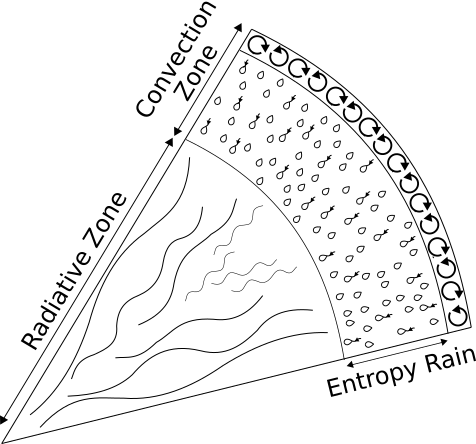
\includegraphics[width=0.32\textwidth]{./figs/entropy_rain_schematic.png}
	\vspace{-16pt}
	\end{center}
    \caption{
	A schematic of the interior of solar-type stars under the entropy rain hypothesis, where cold droplets of fluid carry the stellar luminosity below a small traditional convective surface layer.
	\label{fig:entropy_rain} }
	\vspace{-16pt}
\end{wrapfigure}

Convection which occurs in the presence of atmospheric density stratification exhibits asymmetrical upflows and downflows.
Upwellings are slow, weak, and wide while downflows are intense, fast, and narrow.
The ``entropy rain'' hypothesis \citep[][]{spruit1997} posits that downflows alone may be sufficiently powerful in stellar envelope convection to transport the stellar luminosity.
Upflows with negligible energy transport would exist alongside these downflows mostly to conserve mass.
This hypothesis, and the nontraditional dynamical form of convection it suggests, could explain the absence of giant cells in observations.
Recent simulations of envelope convection suggest that surface-driven downflows can transport most of the stellar luminosity \citep{kapyla&all2017}, and a modified MLT with entropy rain was recently derived by \citet{brandenburg2016}.
A schematic of the entropy rain picture is shown in Fig.~\ref{fig:entropy_rain}.


\paragraph{Entropy Rain: Individual Raindrops and Incorporation into MESA} 
\begin{wrapfigure}{l}{0.24\textwidth}
	\begin{center}
	\vspace{-28pt}
    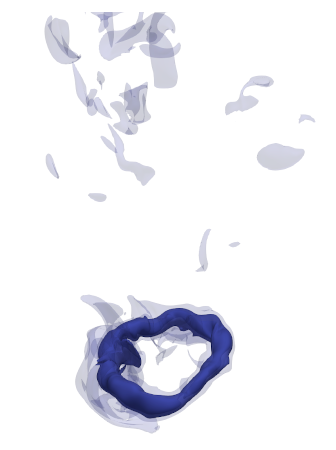
\includegraphics[width=0.22\textwidth]{./figs/turbulent_thermal.png}
	\vspace{-16pt}
	\end{center}
    \caption{
	A 3D visualization of entropy perturbations within the downward-propagating reference frame of a turbulent thermal, which may be the dynamical form of entropy rain.
	\label{fig:thermal} }
	\vspace{-16pt}
\end{wrapfigure}

The entropy rain hypothesis suggests that we should study the nonlocal effects of stellar downflows more carefully.
These downflows may turbulently break up into distinct pieces as they fall and these individual pieces can be modeled as ``thermals.''
Thermals are regions of cold fluid which accelerate due to buoyancy forces and shape themselves into vortex rings; an evolved turbulent thermal is visualized in Fig.~\ref{fig:thermal}.
Thermals are also observed and studied in the Earth's atmosphere \citep{lecoanet&jeevanjee2019}.
In \citet{andersLB2019}, I studied how an atmospheric density stratification affects the size of thermals as they propagate.
I found that thermals compress less than a simple stratification-based estimate would anticipate \citep{brandenburg2016}, and that thermal-like downflows could carry the Sun's luminosity. %, which agrees with the entropy rain hypothesis.

As a postdoctoral scholar at KITP, I will incorporate an MLT with nonlocal heat transport from entropy rain into MESA.
I will study how nonlocal downflow effects alter the stability of the lower convective envelope to learn if entropy rain processes can stabilize the lower convection zone.
Past work \citep{brandenburg2016, andersLB2019} will serve as an excellent starting point for the implementation of MLT into MESA.
While implementing this modified MLT, I will utilize simulations of thermals in Dedalus to determine currently unknown properties of entropy rain, like how much it overshoots into the radiative zone.


\section*{\textbf{Coupling Global Simulations and 1D models}}
Some modern studies seek to remove the need for parameterizations like MLT by coupling 1D stellar structure models with fully convective, three-dimensional (3D) global simulations.
Recently, to great success, \citet{jorgensen&weiss2019} coupled 1D models to previously-computed 3D spherical shell simulations of convection in thin, near-surface layers.
Such a coupling has not yet been performed for deep convection, where most disagreements between simulations and observations occur \citep[the Convective Conundrum,][]{hanasoge&all2015}.

\paragraph{Global Scale Convection: Relaxed Dynamics}
In near-surface shells, the convective overturn timescale is very similar to the local Kelvin-Helmholtz (KH) timescale of atmospheric equilibration.
However, in deep, turbulent convection, many overturn timescales pass during one KH timescale; simulations with deep convection therefore must evolve through a long and scientifically-uninteresting thermal rundown before convective statistics can be sampled.
Creating simulations of deep convection for arbitrary stars which can be coupled with 1D models is therefore too computationally expensive using traditional timestepping techniques.
In \citet{anders&all2018}, I found a mechanism for fast-forwarding through the KH timescale in a simple convective system.
I verified that my fast-forwarding procedure produced the same results as standard timestepping techniques to within 1\%.
This accuracy was achieved using an order of magnitude fewer cpu-hours than traditional techniques.
As a KITP scholar, I will extend my PhD accelerated evolution method \citep{anders&all2018} by creating and validating a generalized public module which rapidly equilibrates mean thermodynamic profiles and flows in global simulations of deep convection.
I will use Dedalus, which can accurately simulate deep convective motions in global domains that include the origin at $r = 0$ \citep[as visualized in Fig.~\ref{fig:mdwarf}, and tested in][]{lecoanet&all2019}, to test the accuracy of this tool.
%This module will effectively take KH-size timesteps by reading in statistical measures from unequilibrated convection and solving for an equilibrated mean state.
%Researchers simulating global convection using arbitrary codes will be able to use this module to rapidly equilibrate simulations with state-of-the-art turbulent dynamics.
%Statistics of deep convection can be sampled from these converged states and coupled with 1D models in the same manner as \citet{jorgensen&weiss2019} coupled simulations of surface convection.

\begin{wrapfigure}{r}{0.3\textwidth}
	\begin{center}
	\vspace{-16pt}
    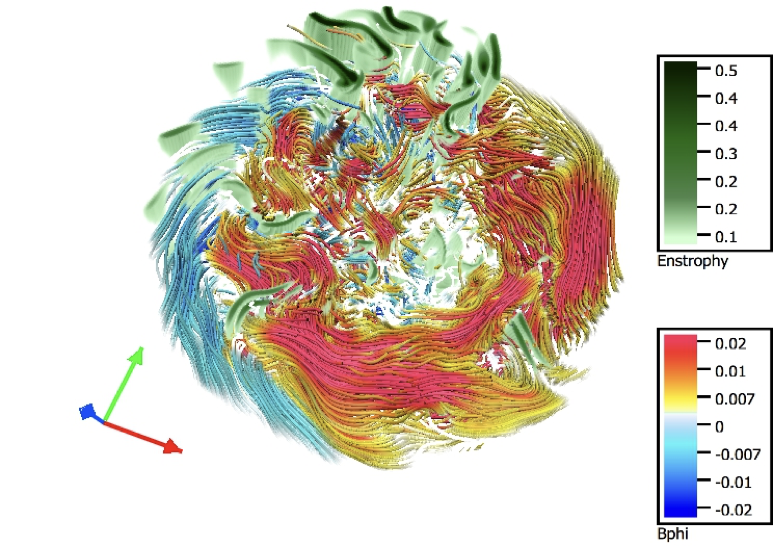
\includegraphics[width=0.28\textwidth]{./figs/mdwarf.png}
	\vspace{-16pt}
	\end{center}
    \caption{A volume rendering of a global dynamo simulation in Dedalus.
	Enstrophy, or the magnitude of vorticity, is shown in green.
	Red and blue lines denote the magnitude and direction of azimuthal magnetic field.
	\label{fig:mdwarf} }
	\vspace{-16pt}
\end{wrapfigure}

\paragraph{Benchmark Main Sequence Models with 3D Convection}
As a KITP scholar, I will couple relaxed global simulations of convection in Dedalus with 1D MESA models to create benchmark structure profiles which are informed by sampled statistics of 3D convection.
Stellar structure is fairly time-stationary over many KH timescales during the main sequence.
As a result, a suite of main-sequence stellar structure profiles which are informed by statistics from convective simulations can be feasibly constructed.
I will create a widely-available public module which couples MESA and 3D global simulations in Dedalus.
This module will take MESA profiles, locate regions of convection in those profiles, and then create simulations (full spheres or spherical shells) of those regions.
Using the previously-developed accelerated evolution tool, these simulations will be forced towards thermal convergence.
Then, the stellar structure profile will be self-consistently updated based on the true measured convective dynamics.
I will compare stellar structure profiles which are built using true convective statistics to those which are built using parameterizations like MLT.
I am particularly curious to see how the dynamical regime of the global simulations affects the full structure of a star.
For example, \citet{featherstone&hindman2016} have shown that rotational effects can mask giant cells in global simulations, and understanding how rotational masking of giant cells -- or masking of giant cells by entropy rain -- is crucial to solving the Convective Conundrum.

\section*{\textbf{Perspectives \& the road forward}}
With more than $10^4$ asteroseismic target stars currently available and an estimated $10^6$ available by 2030 \citep{huber&all2019}, it is critical that we solve the Convective Conundrum to make the most of this wealth of data.
It is clear that our understanding of stellar convection is flawed, but the degree to which this flawed understanding affects asteroseismic measurements is not yet clear.
These studies proposed here will not only help to explore possible solutions to the Convective Conundrum, but will also quantify the amount of error that imperfect convective models like MLT introduce into stellar structure codes.
The successful completion of this work will furthermore provide a set of stellar structure models which are built on sampled convective statistics which observers could utilize in asteroseismic inversions going forward.
I look forward to the opportunity to explore these and other problems with you as I carry on the KITP's excellent research tradition while making lasting contributions towards solving the Convective Conundrum.

\bibliographystyle{yahapj}
\bibliography{biblio}
\end{document}
